\documentclass{article}
\usepackage{listings}
\usepackage{graphicx}
\usepackage[slovene]{babel}
\usepackage{color}
\usepackage{amsmath}
\usepackage{amssymb}
\usepackage{amsfonts}
\usepackage[usenames,dvipsnames]{xcolor}
\usepackage[hidelinks]{hyperref}
\usepackage{subcaption}
\usepackage{float}
\usepackage{rotating} 
\usepackage{hyperref}
\usepackage{caption}
\usepackage{siunitx}
\usepackage[margin=3cm]{geometry}
\graphicspath{{./images/}}

\setlength{\parindent}{0pt}

\renewcommand{\Re}{\mathop{\rm Re}\nolimits}
\renewcommand{\Im}{\mathop{\rm Im}\nolimits}
\newcommand{\Tr}{\mathop{\rm Tr}\nolimits}
\newcommand{\diag}{\mathop{\rm diag}\nolimits}
\newcommand{\dd}{\,\mathrm{d}}
\newcommand{\ddd}{\mathrm{d}}
\newcommand{\ii}{\mathrm{i}}
\newcommand{\lag}{\mathcal{L}\!}
\newcommand{\ham}{\mathcal{H}\!}
\newcommand{\four}[1]{\mathcal{F}\!\left(#1\right)}
\newcommand{\bigO}[1]{\mathcal{O}\!\left(#1\right)}
\newcommand{\sh}{\mathop{\rm sinh}\nolimits}
\newcommand{\ch}{\mathop{\rm cosh}\nolimits}
\renewcommand{\th}{\mathop{\rm tanh}\nolimits}
\newcommand{\erf}{\mathop{\rm erf}\nolimits}
\newcommand{\erfc}{\mathop{\rm erfc}\nolimits}
\newcommand{\sinc}{\mathop{\rm sinc}\nolimits}
\newcommand{\rect}{\mathop{\rm rect}\nolimits}
\newcommand{\ee}[1]{\cdot 10^{#1}}
\newcommand{\inv}[1]{\left(#1\right)^{-1}}
\newcommand{\invf}[1]{\frac{1}{#1}}
\newcommand{\sqr}[1]{\left(#1\right)^2}
\newcommand{\half}{\frac{1}{2}}
\newcommand{\thalf}{\tfrac{1}{2}}
\newcommand{\pd}{\partial}
\newcommand{\Dd}[3][{}]{\frac{\ddd^{#1} #2}{\ddd #3^{#1}}}
\newcommand{\Pd}[3][{}]{\frac{\pd^{#1} #2}{\pd #3^{#1}}}
\newcommand{\avg}[1]{\left\langle#1\right\rangle}
\newcommand{\norm}[1]{\left\Vert #1 \right\Vert}
\newcommand{\braket}[2]{\left\langle #1 \vert#2 \right\rangle}
\newcommand{\obraket}[3]{\left\langle #1 \vert #2 \vert #3 \right \rangle}
\newcommand{\hex}[1]{\texttt{0x#1}}

\begin{document}

\title{Matematično-fizikalni praktikum \\[3mm] \large Naloga 12}
\author{Luka Papež}
\date{30.\ junij 2025}

\begin{center}
    
\includegraphics[width=8cm]{logo-fmf.png}
\end{center}

{
    \let\newpage\relax
    \maketitle
}

\newpage
\section{Naloga}
Na spletni učilnici je na voljo material (koda, vzorci) za 
ločevanje dogodkov Higgsovega bozona od ostalih procesov ozadja. V naboru simuliranih 
dogodkov je 21 karakteristik (zveznih kinematičnih lastnosti), katerih vsaka 
posamezno zelo slabo loči 'signal' od ozadja, z uporabo BDT ali (D)NN, pa lahko tu dosežemo
zelo dober uspeh.  Na predavanjih smo si ogledali glavne aspekte pomembne pri implementaciji ML, 
kot so  uporaba ustreznih spremenljivk (GIGO), učenje in prekomerno učenje (training/overtraining), 
vrednotenje uspeha metode kot razmerje med učinkovitostjo (efficiency) in čistostjo (precision) 
vzorca (Receiver Operating Characteristic, ROC). Določi uspešnost obeh metod (in nariši ROC) 
za nekaj tipičih konfiguracij BDT in DNN, pri čemer:
\begin{itemize}
  \item Študiraj vpliv uporabljenih vhodnih spremenljivk - kaj, če vzamemo le nekatere?
  \item Študiraj BDT in NN in vrednoti uspešnost različnih nastavitev,  če spreminjaš nekaj konfiguracijskih parametrov
  (npr. število perceptronov in plasti nevronskih mrež pri DNN in število dreves pri BDT). 
\end{itemize}

\noindent{\sl Dodatna Naloga:} Implementiraj distribucije iz ‘playground’ zgleda v BDT (lahko tudi RandomForests) in DNN,
te distribucije so na voljo v vseh popularnih ML paketih (npr. Scikit...).

\section{Teoretični uvod}
Dandanes je uporaba različnih algoritmov strojnega učenja (Machine Learning, ML) v 
znanosti že rutinsko opravilo. Poznamo tri osnovne vrste stojnega učenja:
\begin{itemize}
  \item Nadzorovano učenje (Supervised learning):
  \begin{itemize}
    \item Klasifikacija (Classification): sortiranje v različne kategorije.
    \item Regresija (Regression): modeliranje oz. `fitanje' napovedi.
  \end{itemize}
  \item Nenadzorovano učenje ( npr. sam najdi kategorije).
  \item Stimulirano učenje ( Artificial Intelligence v ožjem pomenu besede).
\end{itemize}
V fiziki (in tej nalogi), se tipično ukvarjamo s prvo kategorijo, bodisi za identifikacijo novih pojavov/delcev/\ldots ali pa za ekstrakcijo napovedi (netrivialnih funkcijskih odvisnosti etc).

ML algoritmi imajo prednost pred klasičnim pristopom, da lahko učinkovito razdrobijo kompleksen problem na enostavne elemente in ga ustrezno opišejo.

Če dodamo malce matematičnega formalizma strojnega učenja: Predpostavi, da imamo na voljo nabor primerov 
\(\mathcal{D}=\left\{\left(\mathbf{x}_{k}, y_{k}\right)\right\}_{k=1 . N},\) kjer je
\(\mathbf{x}_{k}=\left(x_{k}^{1}, \ldots, x_{k}^{M}\right)\) naključno izbrani vektor
 \(M\) lastnosti (karakteristik) in je \(\mathbf{y}_{k} = \left(y_{k}^{1}, \ldots, y_{k}^{Q}\right)\)
 vektor $Q$ ciljnih vrednosti, ki so lahko bodisi binarne ali pa realna 
 števila\footnote{...ali pa še kaj, prevedljive na te možnosti, npr barve\ldots}. 
 Vrednosti \(\left(\mathbf{x}_{k}, \mathbf{y}_{k}\right)\) so neodvisne in porazdeljene po neki
 neznani porazdelitvi \(P(\cdot, \cdot) .\) Cilj ML metode je določiti (priučiti) funkcijo
 \(h: \mathbb{R}^{Q} \rightarrow \mathbb{R}\), ki minimizira pričakovano vrednost \emph{funkcije
 izgube (expected loss)} \[
\mathcal{L}(h)=\mathbb{E}\, L(\mathbf{y}, \mathbf{h}(\mathbf{x})) = \frac{1}{N}\sum\limits_{k=1}^{N} L(\mathbf{y_k}, \mathbf{h}(\mathbf{x_k}))  .\] 
 Tu je \(L(\cdot, \cdot)\)  gladka funkcija, ki opisuje oceno za kvaliteto napovedi, 
 pri čemer so  vrednosti \((\mathbf{x}, \mathbf{y})\)
 neodvisno  vzorčene iz nabora \(\mathcal{D}\) po porazdelitvi \(P\). Po koncu učenja
 imamo torej na voljo funkcijo $\mathbf{h}(\mathbf{x})$, ki nam za nek vhodni nabor vrednosti
 $\mathbf{\hat{x}}$ poda napoved $\mathbf{\hat{y}}=\mathbf{h}(\mathbf{\hat{x}})$, ki ustrezno kategorizira
 ta nabor vrednosti. 
 
 Funkcije $\mathbf{h}$ so v praksi sestavljene iz (množice) preprostih funkcij z (nekaj) prostimi
 parametri, kar na koncu seveda pomeni velik skupni nabor neznanih parametrov in zahteven
 postopek minimizacije funkcije izgube. 
 
 Osnovni gradnik odločitvenih dreves je tako kar stopničasta funkcija $H(x_i-t_i)={0,1}$, ki je enaka
 ena za $x_i > t_i$ in nič drugače in kjer je $x_i$ ena izmed karakteristik in $t_i$ neznani parameter.
Iz skupine takšnih funkcij, ki predstavljajo binarne odločitve lahko skonstruiramo končno uteženo 
funkcijo \[
\mathbf{h}(\mathbf{x})=\sum\limits_{i=1}^{J} \mathbf{a}_{i}\, H(x_i-t_i),\] kjer so $\mathbf{a}_i$ vektorji neznanih uteži. 
Tako $t_i$ kot $\mathbf{b}_i$, lahko določimo v procesu učenja. Nadgradnjo predstavljajo nato \emph{pospešena} odločitvena
drevesa (BDT), kjer nadomestimo napoved enega drevesa z uteženo množico le-teh, tipično dobljeno
v ustreznih iterativnih postopkih (npr. AdaBoost, Gradient Boost ipd.).

Pri nevronskih mrežah je osnovni gradnik t.i. \emph{perceptron}, ki ga opisuje preprosta funkcija
\[h_{w,b}(\mathbf{X})=\operatorname{\theta}\left(\mathbf{w}^{T} \cdot \mathbf{X} + b\right),\]
kjer je $\mathbf{X}$ nabor vhodnih vrednosti, $\mathbf{w}$ vektor vrednosti uteži, s katerimi
tvorimo uteženo vsoto ter $b$ dodatni konstatni premik (bias). Funkcija $\theta$ je preprosta
gladka funkcija (npr. $\arctan$), ki lahko vpelje nelinearnost v odzivu perceptrona. Nevronska
mreža je nato sestavljena iz (poljubne) topologije takšnih perceptronov, ki na začetku
sprejme karakteristiko dogodka $\mathbf{x}$ v končni fazi rezultirajo v napovedi $\mathbf{\hat{y}}$, ki 
mora seveda biti čim bližje ciljni vrednosti $\mathbf{y}$. Z uporabo ustrezne funkcije 
izgube (npr MSE: \(\mathcal{L}(h)=\mathbb{E}\, ||\mathbf{y}-\mathbf{\hat{y}}||^2\)), se problem znova prevede na
minimizacijo, kjer iščemo optimalne vrednosti (velikega) nabora uteži $\mathbf{w}_i$ ter
$b_i$ za vse perceptrone v mreži. Globoke nevronske mreže (DNN) niso nič drugega, kot 
velike nevronske mreže ali skupine le-teh. 

Že namizni računalniki so
dovolj močni za  osnovne računske naloge, obstajajo pa tudi že zelo uporabniku prijazni vmesniki v jeziku Python, na primer:
\begin{itemize}
  \item Scikit-Learn (\emph{scikit-learn.org}): odprtokodni paket za strojno učenje,
  \item TensorFlow (\emph{tensorflow.org}): odprtokodni Google-ov sistem za ML, s poudarkom na globokih nevronskih mrežah 
  ( Deep Neural Networks, DNN) z uporabo vmesnika Keras. Prilagojen za delo na GPU in TPU. 
  \item Catboost: (\emph{Catboost.ai}) : odprtokodna knjižnica za uporabo pospešenih odločitvenih dreves (Boosted Decision Trees, BDT). Prilagojena za delo na GPU.
\end{itemize}

\newpage
\section{Rešitev}
\subsection{Podatki}
Podani podatki so bili pridobljeni s pomočjo metode Monte-Carlo, ki temelji na napovedih standardnega modela. Na voljo je $11M$ podatkov, $400{,}000$ od teh uporabljamo za učne podatke in $100{,}000$ za testne, če ni definirano drugače. Glavni cilj je naučiti algoritem, da loči med signalnimi procesi, ki proizvedejo Higgsov bozon in tistimi, ki ga ne. Za vsak dogodek je na voljo 28 karakteristik: 21 osnovnih kinematičnih spremenljivk in sedem funkcij teh spremenljivk, ki so izpeljane za prepoznavanje med razredoma. Namen razvoja takega modela je iskanje Higgsovega bozona v eksperimentalnih podatkih, z najdbo katerega potrdimo standardni model.


Na sliki \ref{fig:distributions} so prikazane porazdelitve za tri kinematične spremenljivke in eno funkcijo kinematičnih spremenljivk. Izbrane karakteristike tudi predstavljajo vse porazdelitve v podatkih in sicer konstantno, diskretno, normalno in Boltzmannovo. Že iz tega lahko ugibamo, da imajo različne karakteristike različno pomembnost pri ločevanju, kar si bolj natančno ogledamo kasneje. 

\begin{figure}[H]
\centering
\begin{subfigure}{0.4\textwidth}
    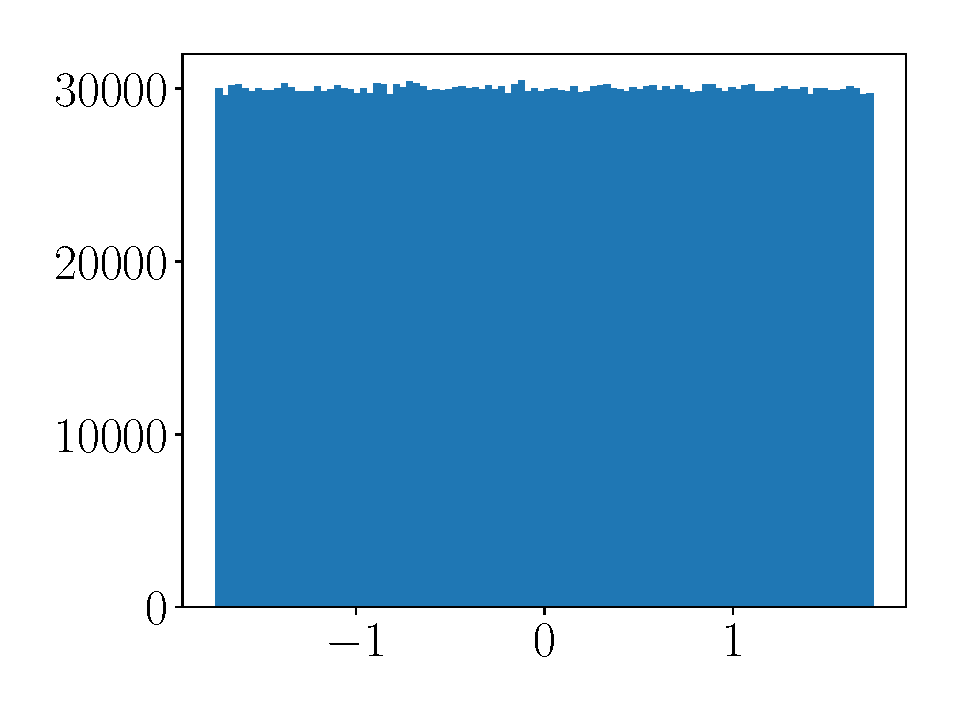
\includegraphics[width=\linewidth]{images/missing-energy-phi.pdf}
	\caption{Porazdelitev kinemati\v{c}ne karakteristike `missing-energy-phi`.}
\end{subfigure}
\begin{subfigure}{0.4\textwidth}
    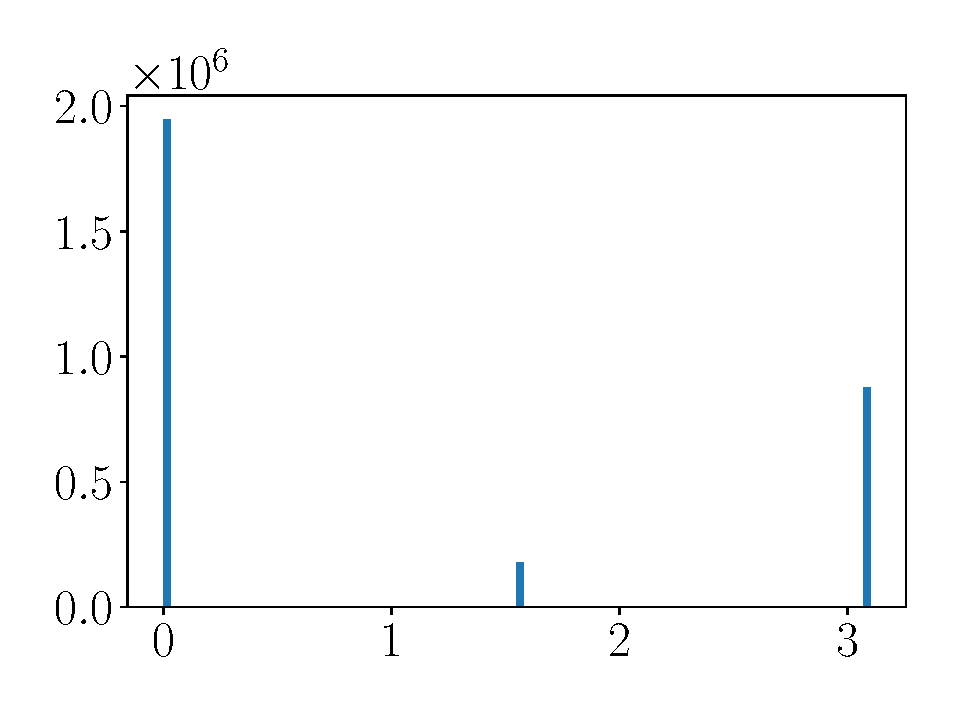
\includegraphics[width=\linewidth]{images/jet_4-b-tag.pdf}
	\caption{Porazdelitev kinemati\v{c}ne karakteristike `jet-4-b-tag`.}
\end{subfigure}

\begin{subfigure}{0.4\textwidth}
    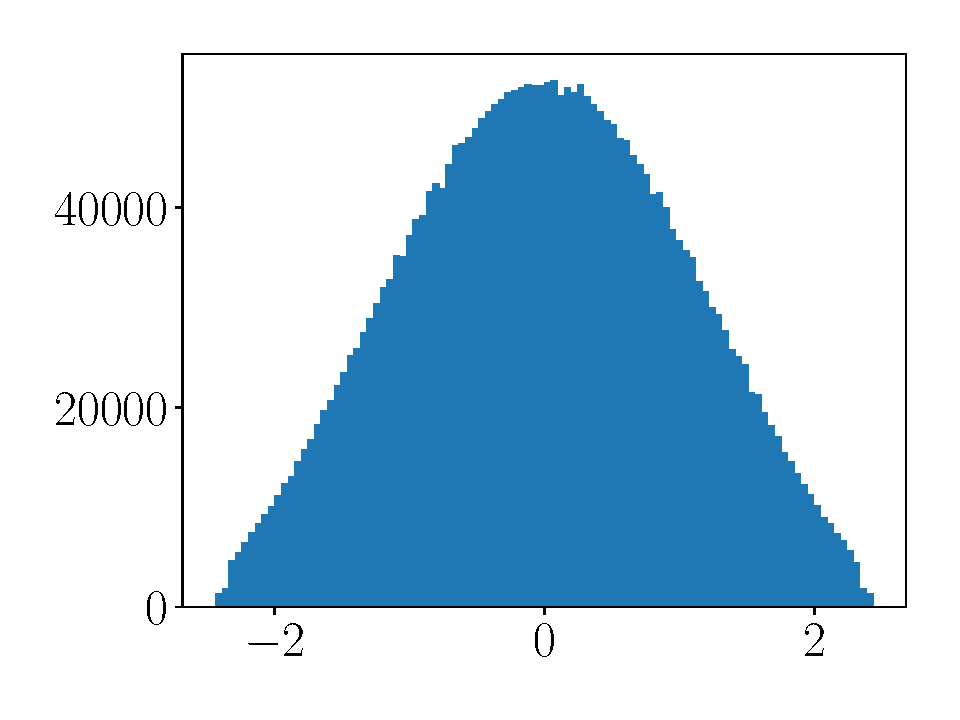
\includegraphics[width=\linewidth]{images/lepton-eta.pdf}
	\caption{Porazdelitev kinemati\v{c}ne karakteristike `lepton-eta`.}
\end{subfigure}
\begin{subfigure}{0.4\textwidth}
    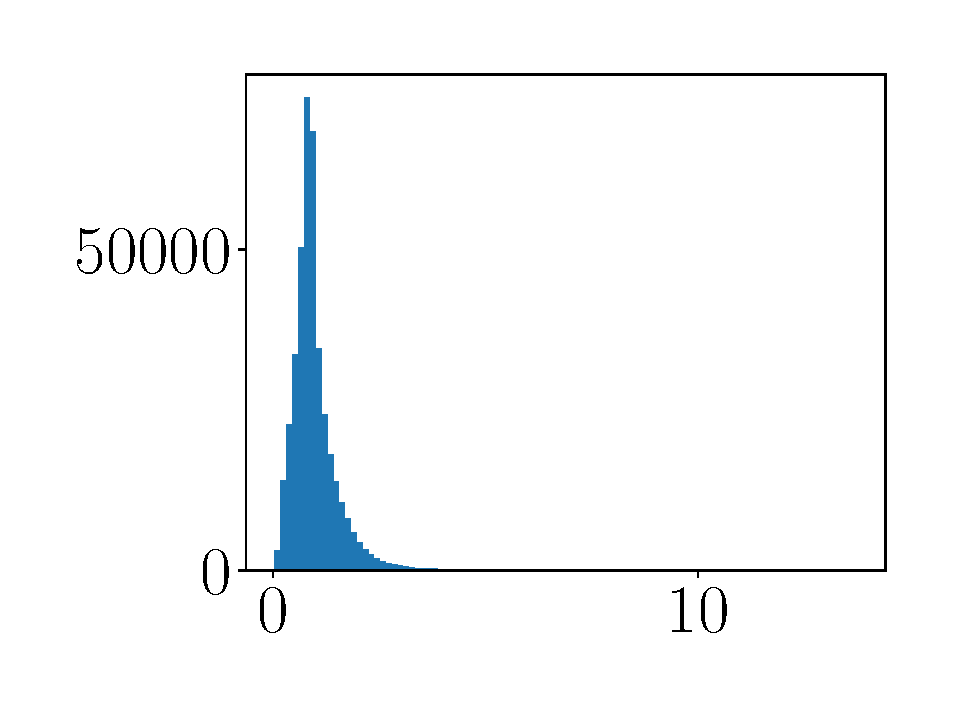
\includegraphics[width=\linewidth]{images/m_bb.pdf}
	\caption{Porazdelitev funkcije kinemati\v{c}nih karakteristik `m-bb`}
\end{subfigure}

\caption{Porazdelitve izbranih karakteristik, ki predstavljajo vse tipe porazdelitev v podatkih.}
\label{fig:distributions}
\end{figure}

Preden pa začnemo z različnimi metodami strojnega učenja si poglejmo še korelacijsko matriko med karakteristikami na sliki \ref{fig:correlation_matrix}. Večinoma so karakteristike med sabo nekorelirane. Najbolj korelirana sta `m-wbb` in `m-wwbb`, z njima pa sta korelirana tudi `m-jj`, ter `m-jjj`, ki sta tudi zelo korelirana medseboj. Omembe vredna sta tudi `jet-1-pt` in `jet-2-pt`, ki sta prav tako korelirana s prej omenjenimi karakteristikma in medseboj. Najbolj negativna korelacija pa je med `jet-1-b-tag` in `jet-2-b-tag`.

\begin{figure}[H]
\centering
	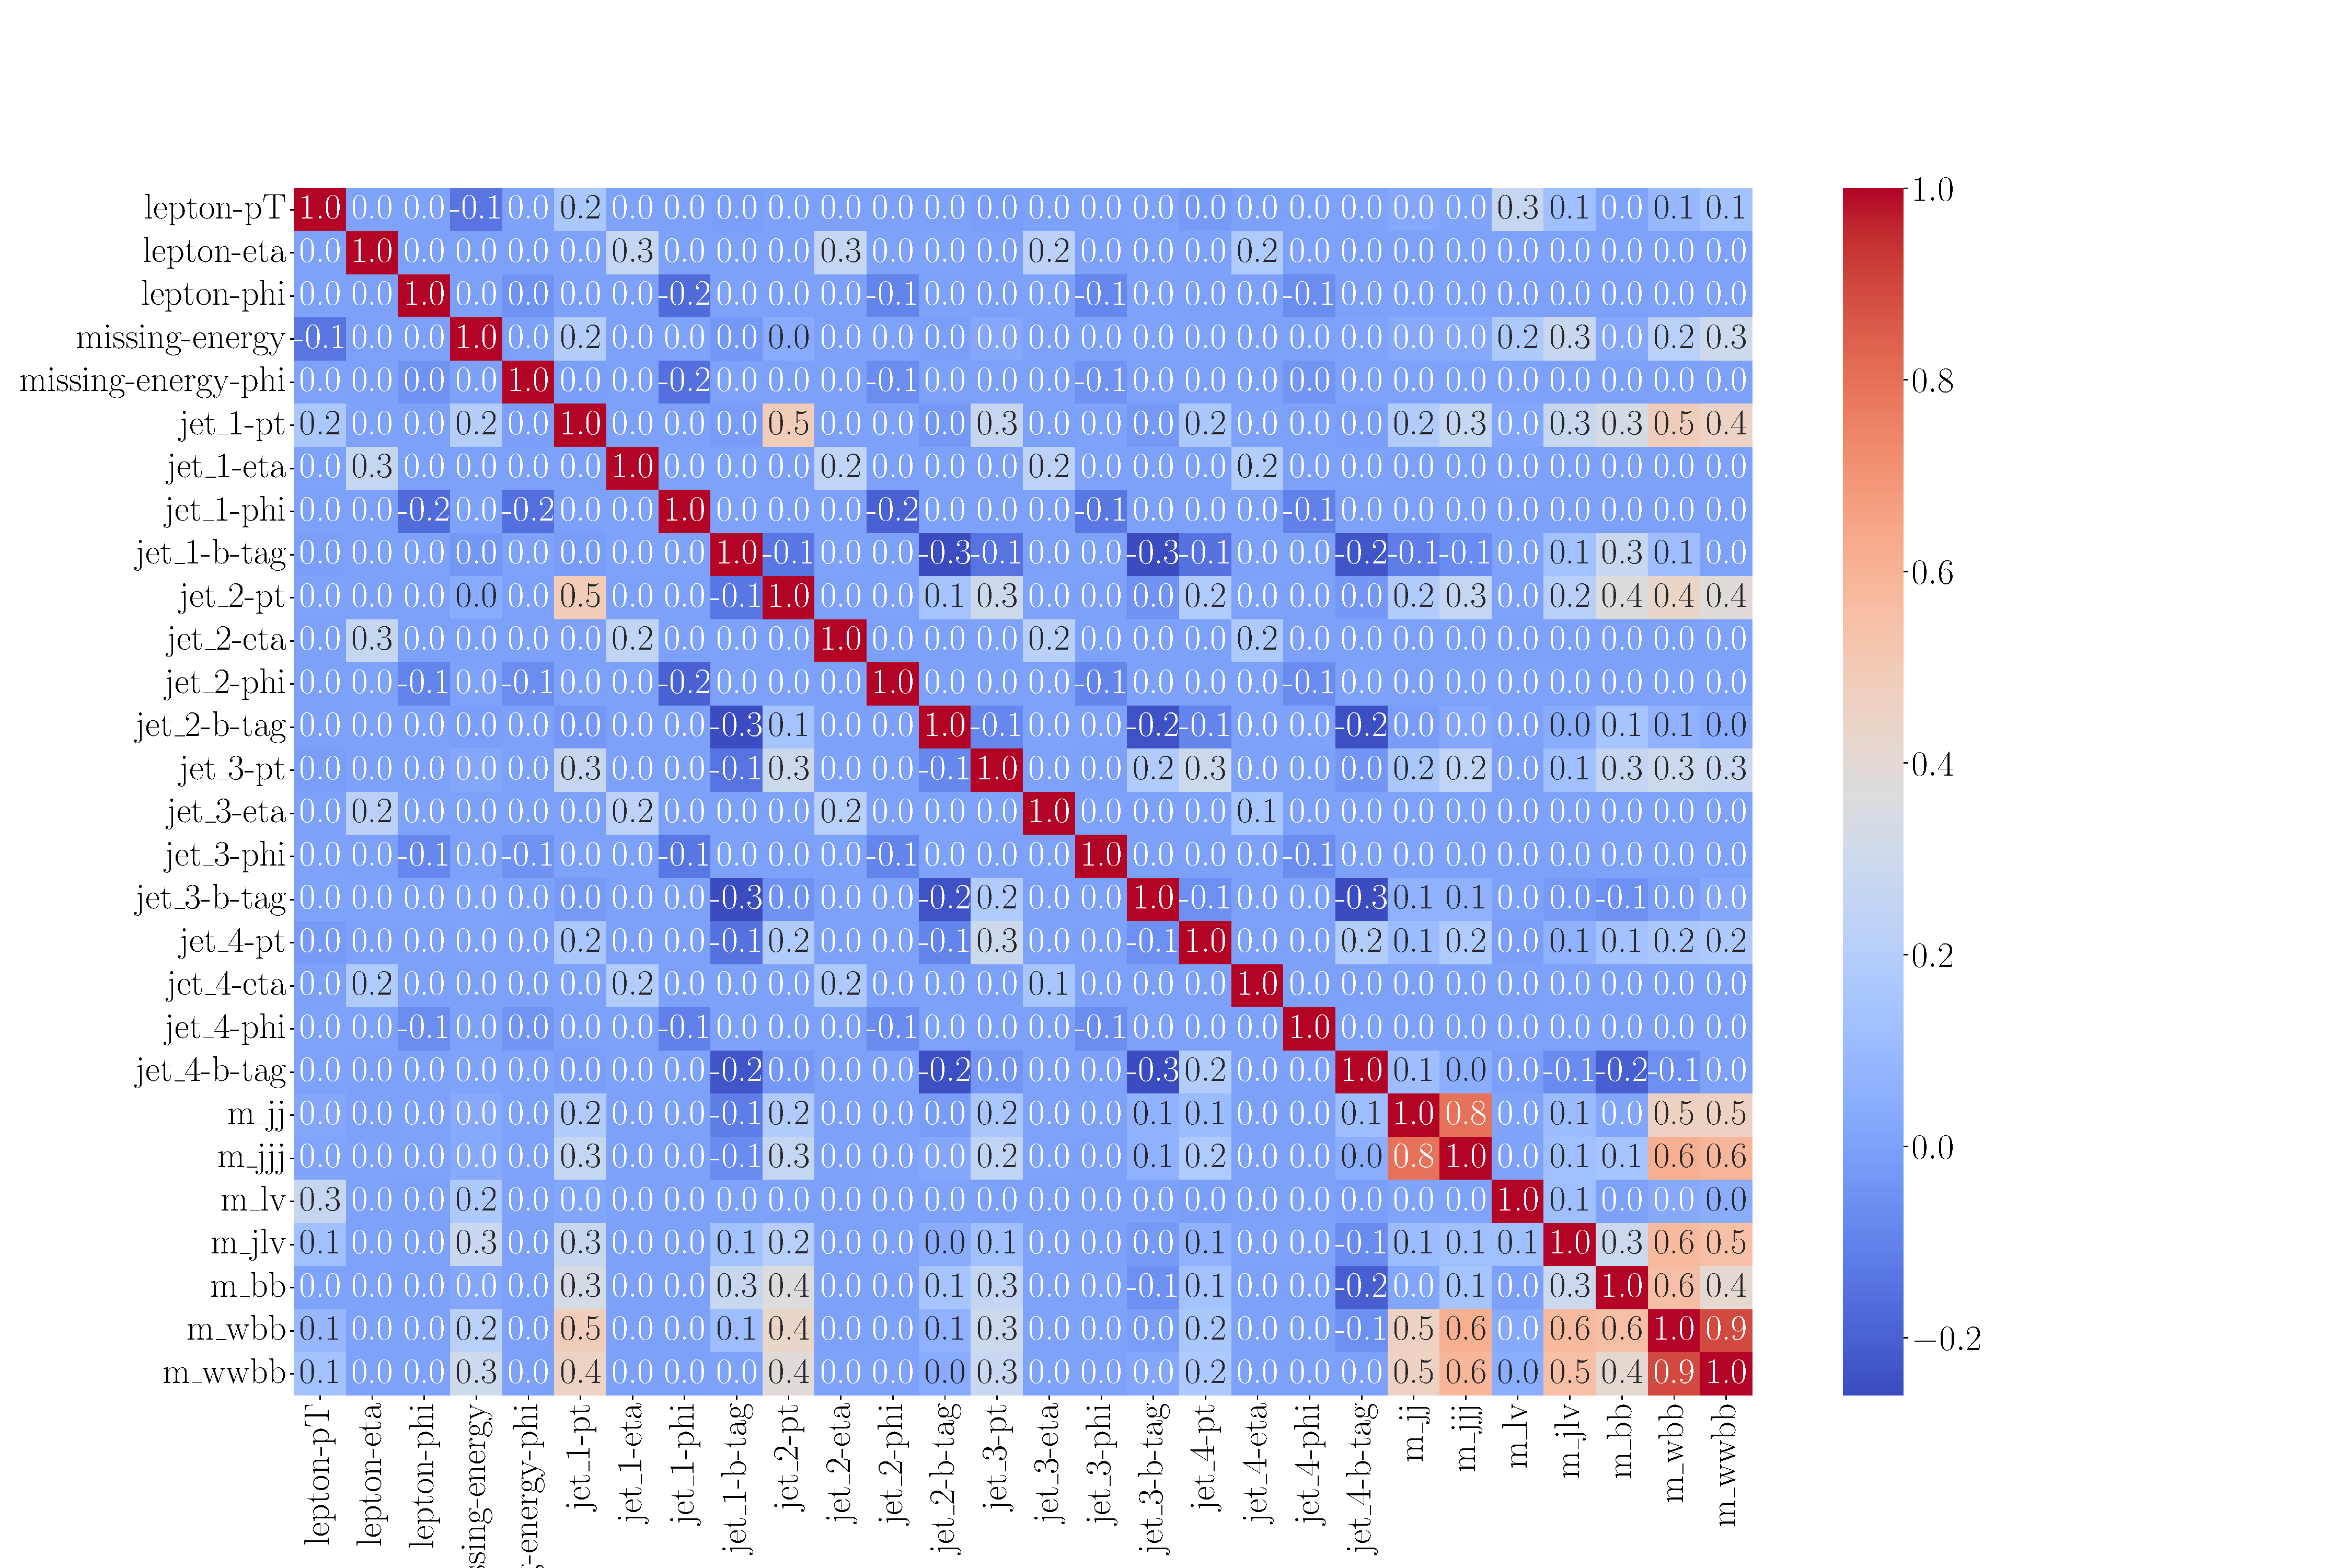
\includegraphics[width=\linewidth]{images/correlation.pdf}
	\caption{Korelacijska matrika karakteristik.}
	\label{fig:correlation_matrix}
\end{figure}

\subsection{Algoritmi strojnega učenja}
K problemu najprej pristopimo s preprosto nevronsko mrežo in odločitvenimi drevesi. Kot že opisano nevronske mreže delujejo na podlagi minimiziranja funkcij izgube s pomočjo spreminjanja uteži. Odločitvena drevesa pa delujejo z maksimiziranjem informacijskega pribitka s pomočjo ločevanja podatkov. Za ocenjevanje natančnosti modela uporabljamo metriko `Area Under Curve`(AUC), ki kot že ime namiguje je ploščina pod krivuljo `Receiver Operating Characteristic`(ROC). Za risanje krivulje uporabimo CatBoost s privzetimi nastavitvami in nevronsko mrežo s pomočjo Tensorflow z dvema plastema po 50 nevronov z aktivacijskima funkcijama ReLU. 
\begin{figure}[H]
\centering
	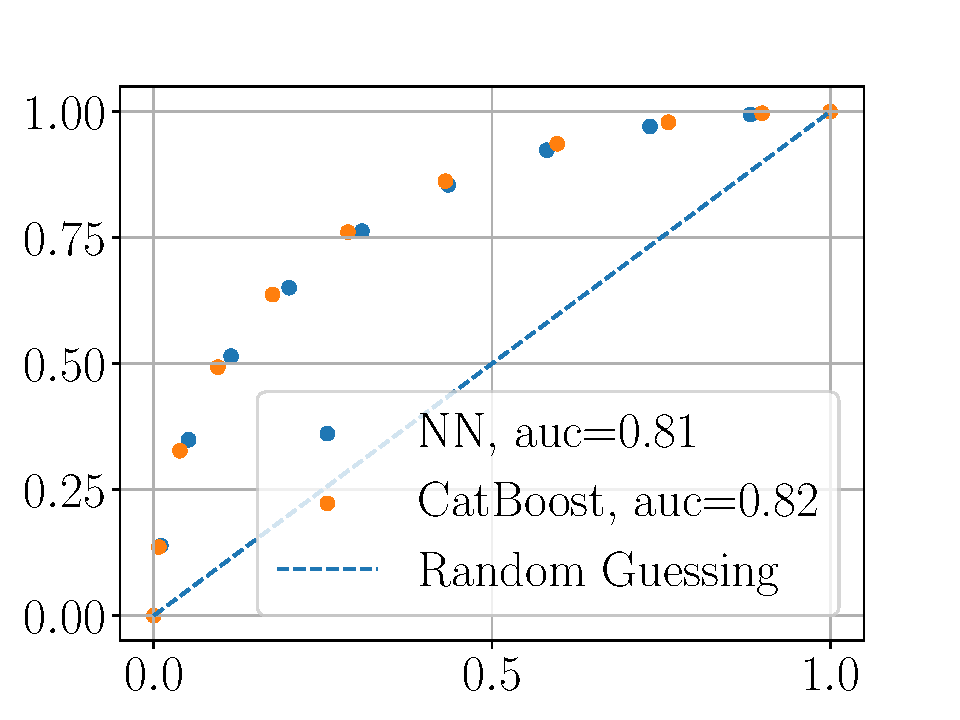
\includegraphics[width=0.5\textwidth]{images/roc.pdf}
	\caption{ROC krivulja za BDT in osnovno nevronsko mrežo.}
	\label{fig:roc}
\end{figure}
Iz slike \ref{fig:roc} opazimo, da sta oba modela primerljiva. Nevronska mreža doseže AUC $0.81$, CatBoost pa $0.82$ torej sta precej boljša od naključnega ugibanja. 
\subsubsection{Nevronske mreže}
Da izboljšamo rezultate prve preproste nevronske mreže je intuitiven proces, da jo povečamo. Za enkrat obdržimo le dve plasti, a ju povečamo, kot je opisano v tabeli \ref{tab:model1}.

\begin{table}[H]
\centering
\begin{tabular}{|l|c|r|}
\hline
\textbf{Plast (tip)}       & \textbf{Oblika izhoda} & \textbf{Param \#} \\
\hline
dense (Dense + ReLU)       & (None, 256)            & 7,168             \\
dense\_1 (Dense + ReLU)    & (None, 64)             & 16,384            \\
dense\_2 (Dense + Sigmoid) & (None, 1)              & 65                \\
\hline
\end{tabular}
\caption{Opis plasti modela 1.}
\label{tab:model1}
\end{table}
Kljub povečanju modela je AUC ostal enak $0.81$. Spomnimo se, da je osnovna vloga nevronskih mrež minimiziranje funkcije izgube, da bolje razumemo kaj se je zgodilo narišimo kako se spreminja funkcija izgube učenja in validacije na sliki \ref{fig:overfitting}. Opzimo, da se validacijska funkcija izgube okoli desetega epoha loči od funkcije izgube učenja. Ta pojav se imenuje `overfitting` in se zgodi, ko je nevronska mreža dovolj velik, da si `zapomni` točne karakteristike vhodnih podatkov.	
\begin{figure}[H]
\centering
	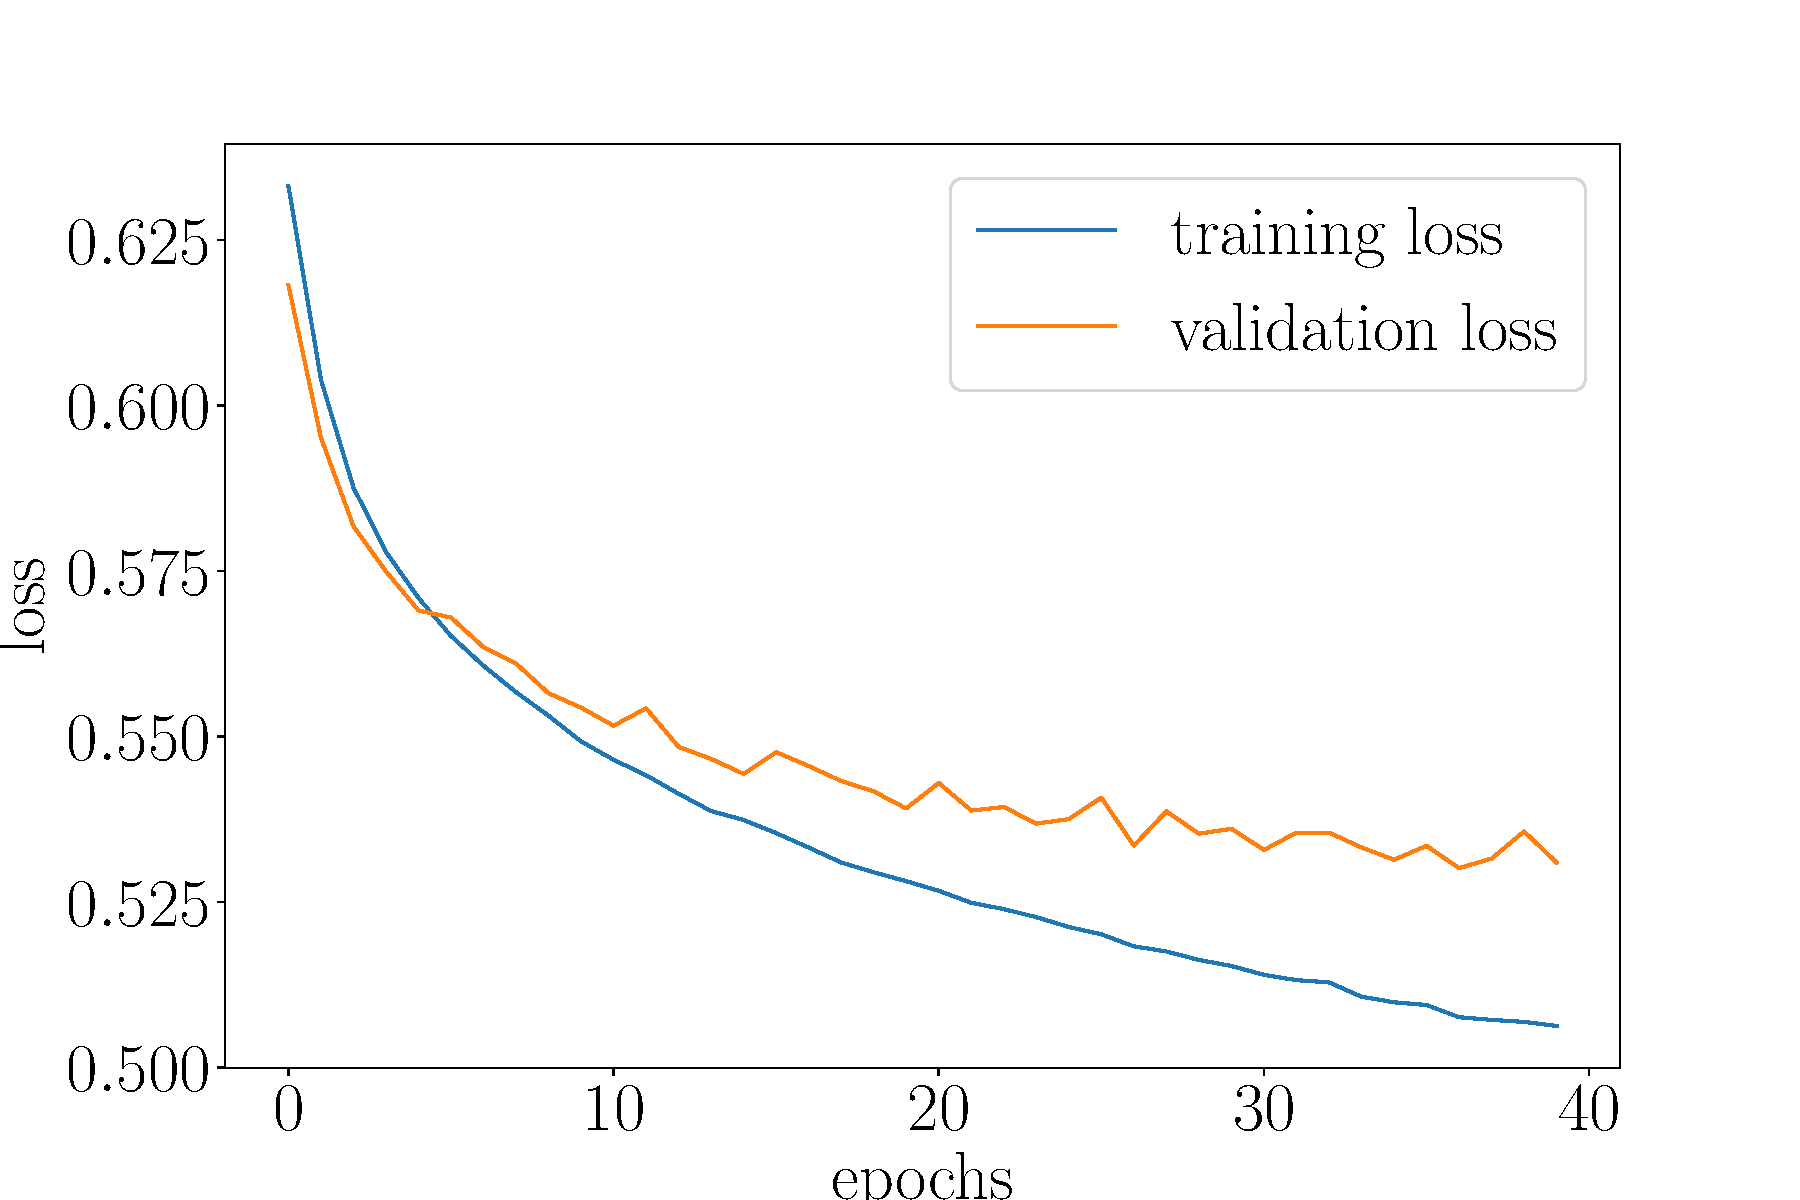
\includegraphics[width=0.5\textwidth]{images/overfittingloss.pdf}
	\caption{Funkcija izgube učenja in validacije modela 1.}
	\label{fig:overfitting}
\end{figure}
V izogib temu pojavu dodamo nevronski mreži tako imenovano plast `Dropout`, ki med učenjem naključno izklopi del uteži in s tem prepreči, da nevronska mreža uporabi specifične uteži za specifične izhode. Poleg tega dodamo še plast `BatchNormalization`, ki normalizira in centrira podatke okoli nič in doda dva nova parametra za učenje, ki popravita morebitno škodo, ki smo jo storili z normalizacijo. Točen vrstni red plasti je na voljo v tabeli \ref{tab:model2}. 
\begin{table}[H]
\centering
\begin{tabular}{|l|c|r|}
\hline
\textbf{Plast (tip)} & \textbf{Oblika izhoda} & \textbf{Param \#} \\
\hline
BatchNormalization		& (None, 28)		   & 112			   \\
Dense + ReLU           & (None, 256)           & 7,168             \\
BatchNormalization     & (None, 256)           & 1,024             \\
Dropout                & (None, 256)           & 0                 \\
Dense + ReLU           & (None, 64)            & 16,384            \\
BatchNormalization     & (None, 64)            & 256               \\
Dense + Sigmoid        & (None, 1)             & 65                \\
\hline
\end{tabular}
\caption{Opis plasti modela 2.}
\label{tab:model2}
\end{table}
Kot je razvidno iz slike \ref{fig:loss} je to rešilo problem `overfittanja` kot nam pove tudi AUC, ki se je rahlo izboljšal na $0.835$. Zanimiva opazka na novem grafu pa je, da je funkcija izgube učenja večja od validacijske. Intuitivno in tudi običajno praktično sta velikosti ravno obratni. Razlog za to spremembo je v plasti `Dropout`, ki deluje le med učenjem. Pri izračunu validacijske funkcije izgube so namreč vključene vse uteži in s tem nevronska mreža deluje bolje oziroma ima manjšo funkcijo izgube.
\begin{figure}[H]
\centering
	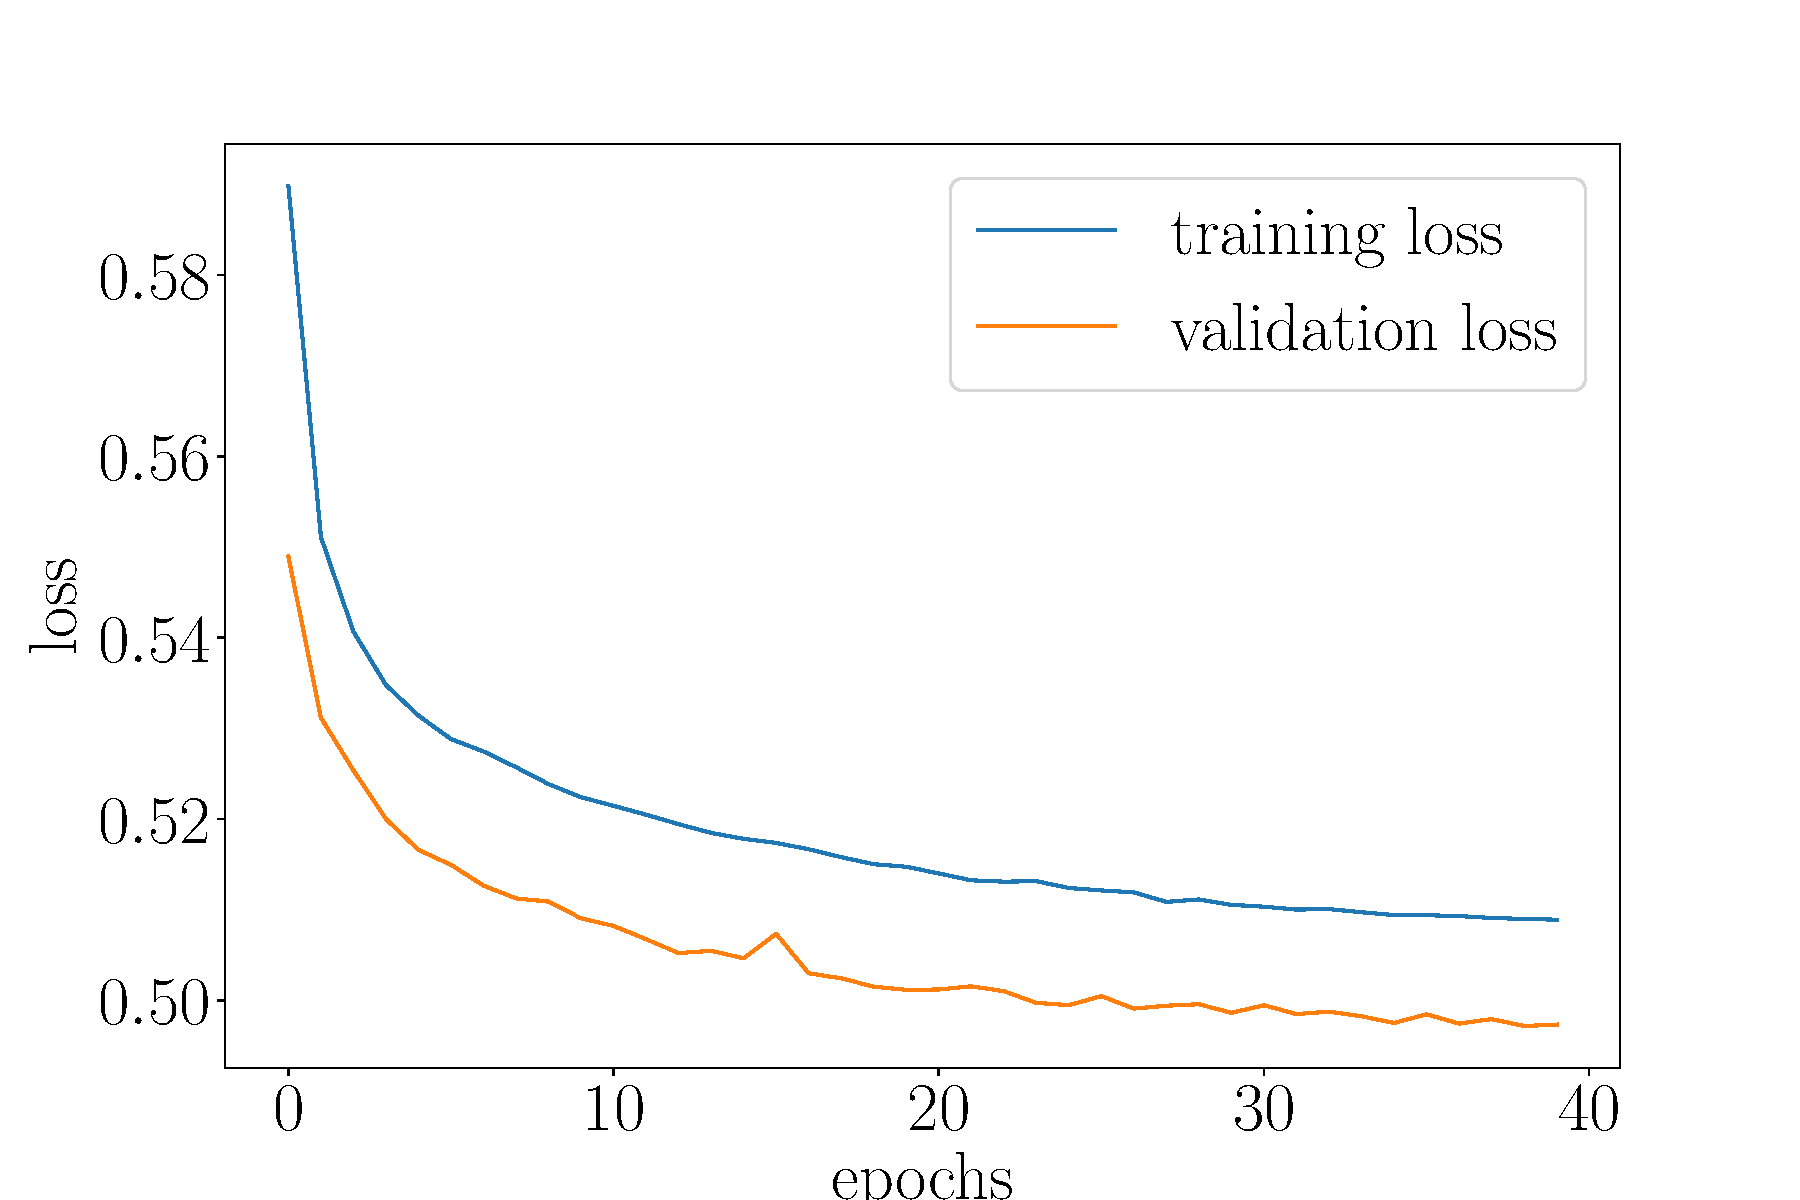
\includegraphics[width=0.5\textwidth]{images/normalloss.pdf}
	\caption{Funkcija izgube učenja in validacije modela 2.}
	\label{fig:loss}
\end{figure}
V naslednjem koraku povečamo število plasti nevronske mreže. To omogoči več zaporednih operacij na podatkih in poveča kompleksnost učenja. Tako pripravimo model v tabeli \ref{tab:model3} in pridemo do rezultata AUC $0.84$. Razlog v majhnem uspehu je pomanjkanje podatkov potrebnih za velikost mreže. Za nadaljnje primere povečamo količino učnih podatkov na $5M$ in testnih na $500{,}000$. To precej podaljša hitrost učenja in po $1000$ epohih se ustali na AUC $0.865$ že po $100$ epohih pa je na $0.86$.
\begin{table}[H]
\centering
\begin{tabular}{|l|l|l|}
\hline
\textbf{Plast (tip)}         & \textbf{Oblika izhoda} & \textbf{Param \#} \\
\hline
BatchNormalization           & (None, 28)   & 112     \\
Dense + ReLU                 & (None, 256)  & 7,168   \\
BatchNormalization           & (None, 256)  & 1,024   \\
Dense + ReLU                 & (None, 128)  & 32,768   \\
BatchNormalization           & (None, 128)  & 512   \\
Dropout                      & (None, 128)  & 0       \\
Dense + ReLU                 & (None, 64)   & 8,192  \\
BatchNormalization           & (None, 64)   & 256     \\
Dense + ReLU                 & (None, 64)   & 4,096  \\
Dense + Sigmoid              & (None, 1)    & 65      \\
\hline
\end{tabular}
\caption{Povzetek arhitekture modela 3.}
\label{tab:model3}
\end{table}
Preden si pogledamo še nevronsko mrežo uporabljeno v članku \cite{Baldi:2014kfa} dodamo modelu 3 avtoenkoder. Avtoenkoder je nevronska mreža sestavljena iz treh komponent, prva je enkoder, kompresnik in dekoder. Prva plast sprejme za vhod podatke za učenje, ki so nato kompresirani na definirano velikost, ponavadi manjšo od števila vhodnih karakteristik. Dekoder nato kompresirane podatke poskuša čim bolj približati vhodnim. Za treniranje avtoenkoderja je potrebno tudi uporabiti funkcijo izgube `mean square error`, ki je kvadrat razlike med vhodom in izhodom. Ko končamo s treniranjem avtoenkoderja, uporabimo enkodersko komponento, s katero kompresiramo vhodne karakteristike, kar nato podamo preostanku modela.

Ta pristop z autoenkoderjem v tabeli \ref{tab:autoencoder}, kjer kompresiramo na velikost $15$, se ni izkazal za preveč uspešnega in je vrnil vrednost AUC $0.826$, ki je precej manjša od prejšnje. Iz tega lahko privzamemo, da kompresiranje ni bilo preveč učinkovito, ter smo izgubili nekaj informacije.
\begin{table}[H]
\centering
\begin{tabular}{|l|l|r|}
\hline
\textbf{Plast (tip)}         & \textbf{Oblika izhoda} & \textbf{Param \#} \\
\hline
Input                        & (None, 28)             & 0           \\
BatchNormalization           & (None, 28)             & 112         \\
Dense + ReLU               & (None, 50)             & 1,450       \\
BatchNormalization           & (None, 50)             & 200         \\
Dropout                      & (None, 50)             & 0           \\
Dense + ReLU               & (None, 15)             & 765         \\
BatchNormalization           & (None, 15)             & 60          \\
Dense + ReLU                 & (None, 50)             & 800         \\
BatchNormalization           & (None, 50)             & 200         \\
Dropout                      & (None, 50)             & 0           \\
Dense + Sigmoid              & (None, 28)             & 1,428       \\
Output						 &	(None, 28)            & 0			\\	
\hline
\end{tabular}
\caption{Povzetek arhitekture autoencoderja.}
\label{tab:autoencoder}
\end{table}
Za zaključek poglavja o nevronskih mrežah implementirajmo še nevronsko mrežo iz članka \cite{Baldi:2014kfa}. Ta je implementirana v knjižnici `pylearn2`, ki ni več vzdrževana zato jo prepišemo v `tensorflow`. Glavna razlika med do sedaj treniranimi mrežami in to iz članka je uporaba aktivacijske funkcije `tanh` namesto `ReLU`. Sama mreža pa je tudi precej večja, z vsemi skritimi plastmi velikosti $300$. Natančna arhitektura je na voljo v tabeli \ref{tab:model4}. V članku poročajo o doseženem AUC $0.885$ s treniranjem mreže za $400$ epohov se k temu približamo z $0.875$, kar je tudi najboljši rezultat od vseh dosedanjih mrež.
\begin{table}[H]
\centering
\begin{tabular}{|l|l|r|}
\hline
\textbf{Plast (tip)}         & \textbf{Oblika izhoda} & \textbf{Param \#} \\
\hline
Dense + tanh               & (None, 300)            & 8,700         \\
Dense + tanh               & (None, 300)            & 90,300        \\
Dense + tanh               & (None, 300)            & 90,300        \\
Dense + tanh               & (None, 300)            & 90,300        \\
Dense + Sigmoid               & (None, 1)              & 301           \\
\hline
\end{tabular}
\caption{Povzetek arhitekture modela 4.}
\label{tab:model4}
\end{table}


\subsubsection{Odločitvena drevesa}
Za analizo delovanja odločitvenih dreves uporabimo knjižnico H2O, ki ponuja funkcijo `AutoML`, ki omogoča preprosto primerjavo več oblik strojnega učenja in iskanje optimalnih parametrov. V tabeli \ref{tab:automl} je podana metrika AUC za najboljše modele posameznih algoritmov, ki vsi temeljijo na odločitvenih drevesih. Za najboljšega za dani primer se je izkazal `Gradient Boosting Machine` takoj za njim `XGBoost` in kot zadnji `Random Forest`. Imajo pa pričakovano vsi modeli relativno podobne rezultate. 
\begin{table}[H]
\centering
\begin{tabular}{|l|l|}
\hline
\textbf{Algoritem} & \textbf{AUC} \\ \hline
GBM & 0.8220 \\ \hline
XGBoost & 0.8151 \\ \hline
DRF & 0.8038 \\ \hline
\end{tabular}
\caption{AUC algoritmov najboljših modelov iz `H2O AutoML`.}
\label{tab:automl}
\end{table}
Ta primerjava med modeli pa seveda ni najboljša, saj funkcija `AutoML` ne garantira najboljšega modela vsakega algoritma. Za boljšo primerjavo pristopimo k problemu s tako imenovanim `GridSearch` algoritmom, ki za en algoritem primerja različne vhodne parametre. Za algoritem `RandomForest` smo dobili pričakovane rezultate, kjer `AUC` narašča najprej z globino dreves, sekundarno pa še s številom dreves. Izkazal pa se je tudi za najhitrejši algoritem, ki je vse kombinacije preveril 4min 27s. Algoritma `XGBoost` ter `Gradient Boosting Machine` pa sta vrnila precej nenavadne rezultate. Pri algoritmu `XGBoost` se je za najboljšo izkazala iteracija z najmanjšo globino in največjim številom dreves. Za najslabšo pa najglobja z najmanj drevesi. Bil pa je tudi najpočasnejši algoritem, ki je potreboval za vse kombinacije 13min 31s. `Gradient Boosting Machine` se je ponovno kot pri `AutoML` izkazal za najboljšega z rahlo izboljšanim rezultatom. Vrstni red globine pa je še precej bolj 
zanimiv tokrat je namreč srednja globina na prvem mestu, najglobja na drugem in najbolj plitka na zadnjem. Uporabljen algoritem pa je našel tudi nekaj števil dreves izven specificiranih vrednosti kot na primer najboljšo vrednost s $107$ drevesi. Za vse možne kombinacije pa je potreboval 6min 24s.
\begin{table}[H]
\centering
\begin{minipage}{0.3\textwidth}
\centering
\begin{tabular}{|c|c|c|}
\hline
\textbf{max\_depth} & \textbf{ntrees} & \textbf{AUC} \\
\hline
5.0 & 250.0 & 0.8169 \\
5.0 & 200.0 & 0.8163 \\
10.0 & 50.0 & 0.8154 \\
10.0 & 100.0 & 0.8150 \\
5.0 & 150.0 & 0.8148\\
15.0 & 250.0 & 0.8143 \\
10.0 & 150.0 & 0.8136 \\
15.0 & 200.0 & 0.8129 \\
5.0 & 100.0 & 0.8127 \\
10.0 & 200.0 & 0.8120 \\
10.0 & 250.0 & 0.8108 \\
15.0 & 150.0 & 0.8103 \\
5.0 & 50.0 & 0.8074 \\
15.0 & 100.0 & 0.8072 \\
15.0 & 50.0 & 0.8044 \\
\hline
\end{tabular}
\caption{Algoritem `XGBoost` iz knjižnica `H2O`}
\end{minipage}
\hfill
\begin{minipage}{0.3\textwidth}
\centering
\begin{tabular}{|c|c|c|}
\hline
\textbf{max\_depth} & \textbf{ntrees} & \textbf{AUC} \\
\hline
10.0 & 107.0 & 0.8235 \\
10.0 & 107.0 & 0.8235 \\
10.0 & 107.0 & 0.8235 \\
10.0 & 100.0 & 0.8231 \\
15.0 & 250.0 & 0.8228 \\
15.0 & 200.0 & 0.8217 \\
15.0 & 150.0 & 0.8205 \\
15.0 & 100.0 & 0.8191 \\
10.0 & 50.0 & 0.8178 \\
15.0 & 50.0 & 0.8158 \\
5.0 & 240.0 & 0.8146 \\
5.0 & 200.0 & 0.8133 \\
5.0 & 150.0 & 0.8109 \\
5.0 & 100.0 & 0.8066 \\
5.0 & 50.0 & 0.7978 \\
\hline
\end{tabular}
\caption{Algoritem `Gradient Boosting Machine` iz knjižnice `H2O`}
\end{minipage}
\hfill
\begin{minipage}{0.3\textwidth}
\centering
\begin{tabular}{|c|c|c|}
\hline
\textbf{max\_depth} & \textbf{ntrees} & \textbf{AUC} \\
\hline
15.0 & 250.0 & 0.8046 \\
15.0 & 200.0 & 0.8043 \\
15.0 & 150.0 & 0.8038 \\
15.0 & 100.0 & 0.8033 \\
15.0 & 50.0 & 0.8012 \\
10.0 & 250.0 & 0.7865 \\
10.0 & 200.0 & 0.7863 \\
10.0 & 150.0 & 0.7860 \\
10.0 & 100.0 & 0.7858 \\
10.0 & 50.0 & 0.7841 \\
5.0 & 250.0 & 0.7526 \\
5.0 & 200.0 & 0.7526 \\
5.0 & 150.0 & 0.7522 \\
5.0 & 100.0 & 0.7518 \\
5.0 & 50.0 & 0.7504 \\
\hline
\end{tabular}
\caption{Algoritem `RandomForest` iz knjižnice `H2O`}
\end{minipage}
\caption{Vrednosti AUC algoritmov kot izhod `GridSearch`.}
\end{table}
Algoritem `CatBoost`, ki smo ga uporabili na začetku pa ni na voljo v knjižnici `H2O` zato za primerjavo poženemo še ta algoritem na prej določenih parametrih. Opazimo, da so vrednosti AUC za približno $0.05$ manjše od ostalih algoritmov. Spreminjanje AUC s parametroma pa je podobno tistemu algoritma `RandomForest`, ki intuitivno narašča z velikostjo in številom dreves. 
\begin{table}[H]
	\centering
	\begin{tabular}{|c|c|c|}
	\hline
	\textbf{max\_depth} & \textbf{ntrees} & \textbf{AUC} \\
	\hline
	15 & 250 & 0.7500 \\
	15 & 200 & 0.7486 \\
	15 & 150 & 0.7466 \\
	15 & 100 & 0.7434 \\
	10 & 250 & 0.7390 \\
	15 & 50  & 0.7380 \\
	10 & 200 & 0.7376 \\
	10 & 150 & 0.7355 \\
	10 & 100 & 0.7321 \\
	10 & 50  & 0.7265 \\
	5  & 250 & 0.7216 \\
	5  & 200 & 0.7198 \\
	5  & 150 & 0.7180 \\
	5  & 100 & 0.7148 \\
	5  & 50  & 0.7088 \\
	\hline
	\end{tabular}
	\caption{Vrednosti AUC, algoritma `CatBoost` pri različnih parametrih.}
\end{table}
\newpage
\subsubsection{Izbira karakteristik}
Pomemben del vsake algoritma pa je seveda razumevanje kako algoritem deluje. Dobra metrika za izračun tega je pomembnost karakteristik, ki je ponavadi že na voljo kot vgrajena funkcija pri odločitvenih drevesih. Pri nevronskih mrežah potrebujemo vložiti malo več truda in uporabiti PermutationImportance, ki premeša vrednosti ene karakteristike in s padcem izbrane metrike določi pomembnost. Iz tabel \ref{tab:nnimportance} in \ref{tab:cbimportance} je razvidno, da je večina karakteristik nepomembnih za klasifikacijo. Iz tega lahko zaključimo, da za klasifikacijo zadošča že le nekaj karakteristik. Za primer zadoščajo tudi že vse karakteristike, ki imajo pomembnost večjo od $0.005$.

\begin{table}[H]
\centering
\begin{minipage}{0.48\textwidth}
\centering
\begin{tabular}{l r}
\hline
\textbf{Karakteristika} & \textbf{PermutationImportance} \\
\hline
m\_wwbb & 0.2442 \\
m\_bb & 0.2189 \\
m\_wbb & 0.1657 \\
jet\_1-pt & 0.0661 \\
m\_jjj & 0.0524 \\
m\_jlv & 0.0433 \\
lepton-pT & 0.0298 \\
m\_jj & 0.0236 \\
missing-energy & 0.0206 \\
jet\_2-pt & 0.0165 \\
m\_lv & 0.0077 \\
jet\_1-b-tag & 0.0060 \\
jet\_3-pt & 0.0054 \\
jet\_4-pt & 0.0043 \\
jet\_3-b-tag & 0.0041 \\
jet\_4-b-tag & 0.0036 \\
jet\_2-b-tag & 0.0031 \\
lepton-eta & 0.0006 \\
jet\_2-eta & 0.0002 \\
jet\_3-eta & 0.0002 \\
jet\_4-eta & 0.0002 \\
jet\_1-eta & 0.0001 \\
jet\_3-phi & 0.0000 \\
jet\_2-phi & 0.0000 \\
missing-energy-phi & 0.0000 \\
lepton-phi & 0.0000 \\
jet\_4-phi & 0.0000 \\
jet\_1-phi & 0.0000 \\
\hline
\end{tabular}
\caption{Pomembnost karakteristik nevronske mreže s `PermutationImportance`}
\label{tab:nnimportance}
\end{minipage}
\hfill
\begin{minipage}{0.48\textwidth}
\centering
\begin{tabular}{l r}
\hline
\textbf{Karakteristika} & \textbf{CatBoost Importance} \\
\hline
m\_bb & 0.2331 \\
m\_wwbb & 0.1585 \\
m\_wbb & 0.1023 \\
m\_jjj & 0.0943 \\
m\_jlv & 0.0829 \\
jet\_1-pt & 0.0767 \\
lepton-pT & 0.0568 \\
m\_jj & 0.0350 \\
missing-energy & 0.0333 \\
jet\_2-pt & 0.0228 \\
lepton-eta & 0.0143 \\
jet\_1-b-tag & 0.0124 \\
jet\_3-pt & 0.0121 \\
m\_lv & 0.0112 \\
jet\_1-eta & 0.0111 \\
jet\_4-pt & 0.0101 \\
jet\_2-eta & 0.0060 \\
jet\_3-eta & 0.0056 \\
jet\_2-b-tag & 0.0051 \\
jet\_3-b-tag & 0.0047 \\
jet\_4-b-tag & 0.0047 \\
jet\_4-eta & 0.0044 \\
jet\_3-phi & 0.0006 \\
jet\_2-phi & 0.0005 \\
missing-energy-phi & 0.0005 \\
lepton-phi & 0.0005 \\
jet\_4-phi & 0.0004 \\
jet\_1-phi & 0.0002 \\
\hline
\end{tabular}
\caption{Vgrajen `Feature Importance` algoritma `CatBoost`.}
\label{tab:cbimportance}
\end{minipage}
\end{table}
\subsubsection{Odločitvena meja}
Za konec narišemo še odločitvene meje za CatBoost in nevronsko mrežo. Za namen tega si izberemo dva `playground dataseta` imenovana `moons` in `circles`. Za nevronko mrežo opazimo postopen prehod med klasificiranima razredoma. V `datasetu moons` v spodnjem delu, kjer ni več na voljo podatkov presentljivo meja tudi obdrži ukrivljenost. 
\begin{figure}[H]
    \centering
    \begin{subfigure}{0.48\textwidth}
        \centering
        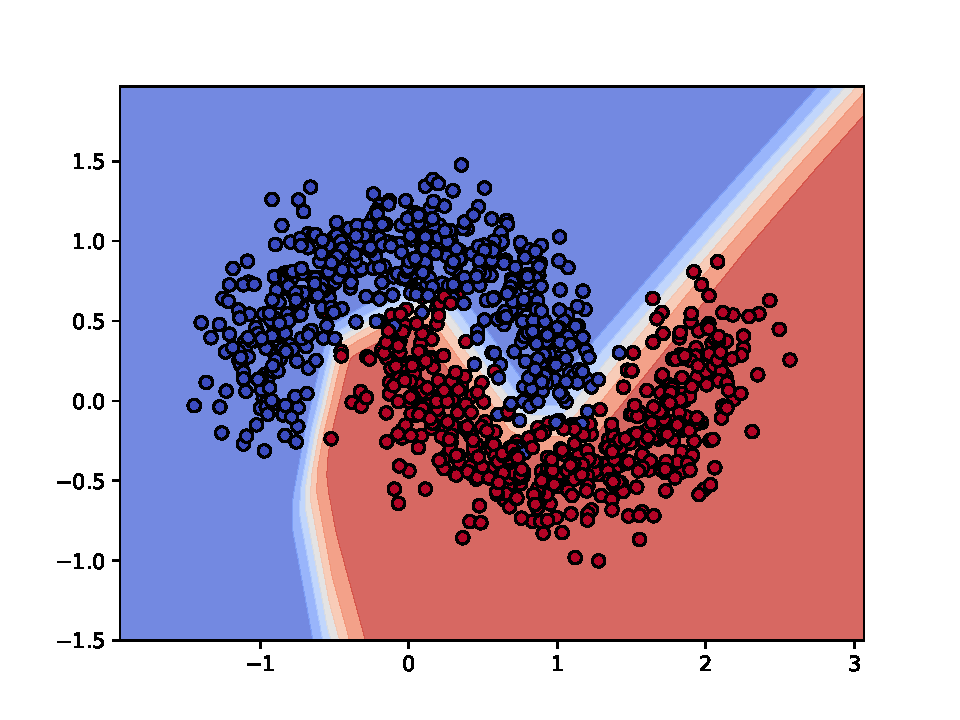
\includegraphics[width=\linewidth]{moonsnn.pdf}
        \caption{Dataset moons}
    \end{subfigure}\hfill
    \begin{subfigure}{0.48\textwidth}
        \centering
        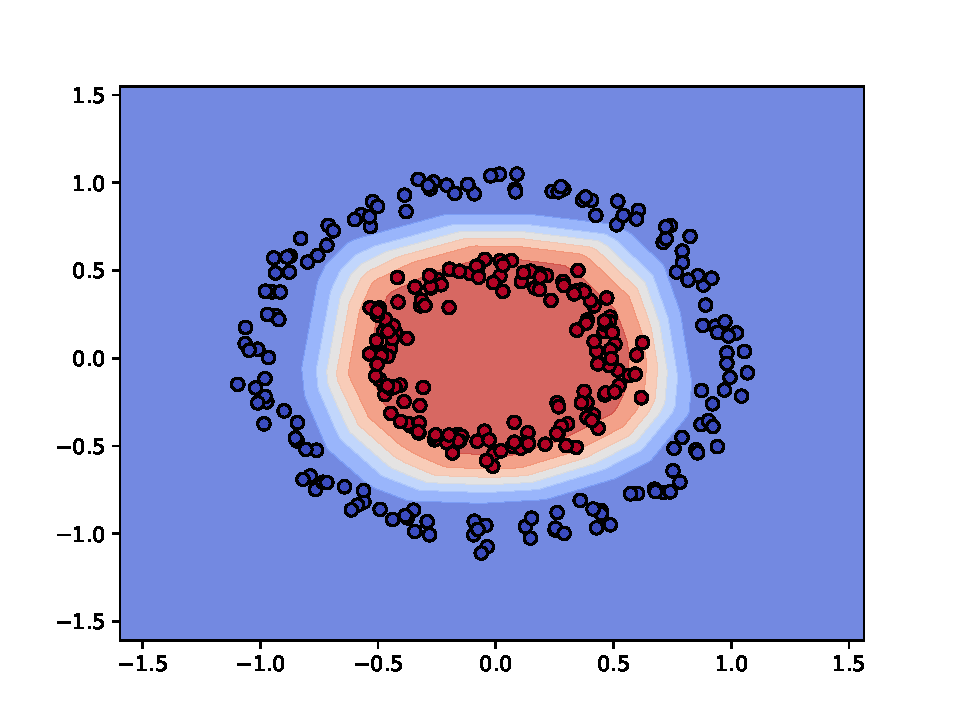
\includegraphics[width=\linewidth]{circlesnn.pdf}
        \caption{Dataset circles}
    \end{subfigure}
    \caption{Odločitveni meji nevronske mreže.}
\end{figure}
Pri algoritmu `CatBoost` je odločitvena meja precej bolj ostra in ni prehodnega območja primerljivega s tistim pri nevronskih mrežah. Rahlo nenavadna je tudi oblika odločitvene meje rdečega razreda, ki spominja bolj na kvadrat kot pa na krog h kateremu močno namigujejo podatki. 
\begin{figure}[H]
    \centering
    \begin{subfigure}{0.48\textwidth}
        \centering
        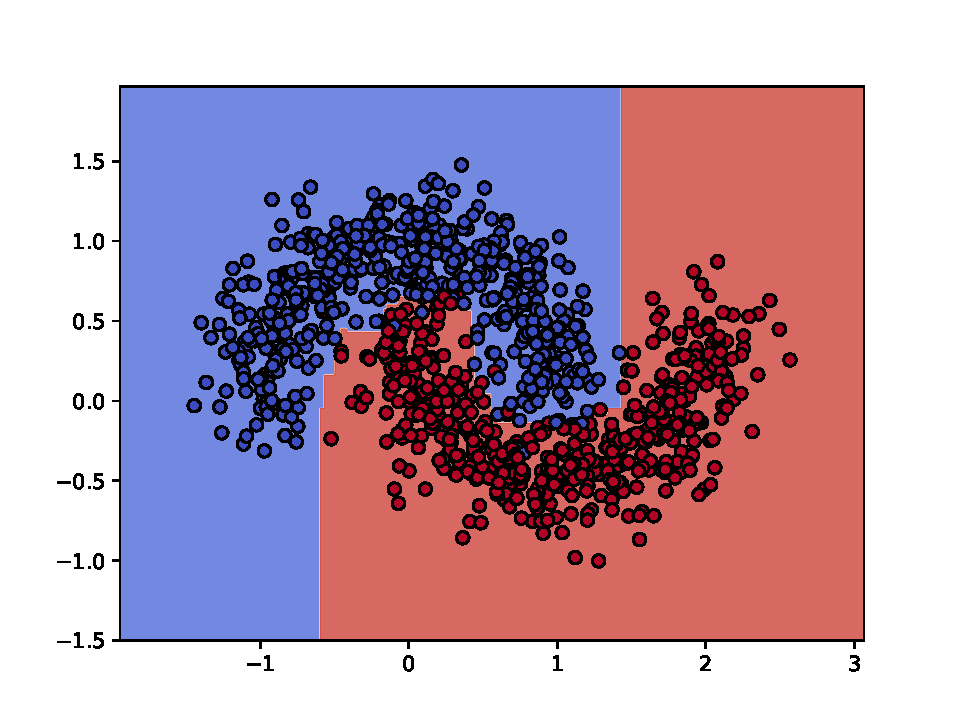
\includegraphics[width=\linewidth]{moonscb.pdf}
        \caption{Dataset moons}
    \end{subfigure}\hfill
    \begin{subfigure}{0.48\textwidth}
        \centering
        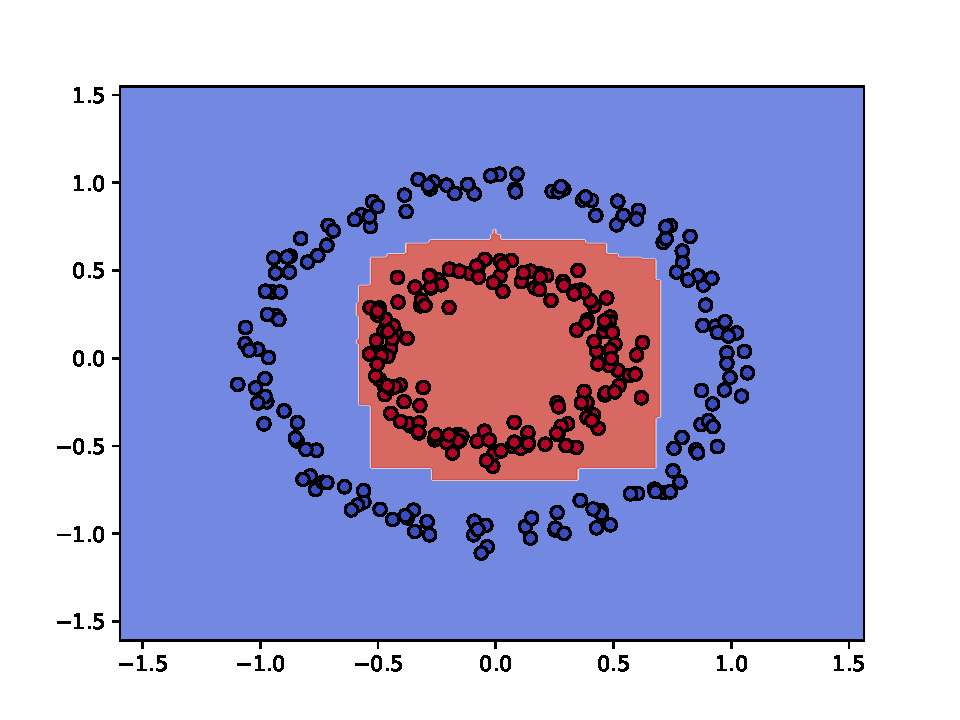
\includegraphics[width=\linewidth]{circlescb.pdf}
        \caption{Dataset circles}
    \end{subfigure}
    \caption{Odločitveni meji algoritma `CatBoost`.}
\end{figure}
\section{Zaključek}
V tej nalogi smo se spoznali z osnovami strojnega učenja na primeru klasificiranja Higgsovega bozona od šuma. Problem smo obravnavali z različnimi konfiguracijami nevronskih mrež in z implementacijo odločitvenih dreves `CatBoost` in nato še z implementacijami iz knjižnice `H2O`, ki omogoča lažjo primerjavo algoritmov.

Za konec pa prilagam še \href{https://journals.aps.org/prresearch/pdf/10.1103/PhysRevResearch.3.L042035}{članek o iskanju invariant s strojnim učenjem}, ki je služil kot inspiracija za moj trenuten projekte. Ideja nevronske mreže je, da za funkcijo izgube uporabiš varianco, katere definicija je rahlo spremenjena z naključnim šumom, da nevronska mreža najde netrivialne invariante iz podanih podatkov.  

\bibliographystyle{plain}
%\bibliography{mybib}

\begin{thebibliography}{1}
 
  
  \bibitem{geron2019hands-on}
  Aur\'{e}lien G\'{e}ron.
  \newblock {\em Hands-on machine learning with Scikit-Learn, Keras, and
    TensorFlow : concepts, tools, and techniques to build intelligent systems}.
  \newblock O'Reilly Media, Inc, Sebastopol, CA, 2019.
  
  \bibitem{prokhorenkova2017catboost}
  Liudmila Prokhorenkova, Gleb Gusev, Aleksandr Vorobev, Anna~Veronika Dorogush,
    and Andrey Gulin.
  \newblock Catboost: unbiased boosting with categorical features, 2017.

  \bibitem{Chen_2016}
  Tianqi Chen and Carlos Guestrin.
  \newblock Xgboost.
  \newblock {\em Proceedings of the 22nd ACM SIGKDD International Conference on
    Knowledge Discovery and Data Mining - KDD ’16}, 2016.

\bibitem{Baldi:2014kfa}
P.~Baldi, P.~Sadowski and D.~Whiteson,
\newblock {\em Searching for Exotic Particles in High-Energy Physics with Deep Learning,}
Nature Commun.\  {\bf 5} (2014) 4308
doi:10.1038/ncomms5308
[arXiv:1402.4735 [hep-ph]].
\end{thebibliography}
\end{document}
